% This file is meant to be a minimal example that displays the
% functions offered by AASTeX v6.3. Created by Ryan Chalener
% (rchallen@knights.ucf.edu)

% Add 'anonymous' option to anonymize for submission
% Note that you need a \nocollaboration command to make
% the anonymous option work.
\documentclass[twocolumn, twocolappendix, numberedappendix, linenumbers]{aastex631}

\usepackage{amsmath}
\usepackage{natbib}
\usepackage{lipsum}

%\bibliographystyle{aasjournal}
\bibliographystyle{aasjournal}

% Unslanted mu, for ``micro'' abbrev.
\DeclareSymbolFont{UPM}{U}{eur}{m}{n}
\DeclareMathSymbol{\umu}{0}{UPM}{"16}
\let\oldumu=\umu
\renewcommand\umu{\ifmmode\oldumu\else$\oldumu$\fi}
\newcommand\micro{\umu}
\renewcommand\micron{\micro m}
\newcommand\microns{\micro m}

% equation shortcut
\newcommand{\beq}{\begin{equation}}
\newcommand{\eeq}{\end{equation}}

% common latin abbreviations
\newcommand{\eg}{{\it e.g.,}}
\newcommand{\ie}{{\it i.e.,}}
\newcommand{\etal}{{\it et~al.}}

% Missions
\newcommand{\Cas}{{\it Cassini}}
\newcommand{\Vgr}{{\it Voyager}}

% misc
\newcommand{\tdex}[1]{$\times 10^{#1}$}  % scientific notation (in text)
\newcommand{\degrees}{$^\circ$}    % degrees (in text)
\newcommand{\Rs}{$R_S$}      % Saturn radii (in text)

\shorttitle{Cassini VIMS Stellar Occultations: Imaging Mode}
\shortauthors{Foster {\em et al.}}

\received{ January 41, 2123}
\revised{  January 42, 2123}
\accepted{ January 43, 2123}
\published{January 44, 2123}
\submitjournal{Journal Name}

\begin{document}

\title{Stellar Occultation Studies of Saturn's Stratosphere I: Imaging Mode}
% List each author and their affiliations
% Brackets are for ORCID
\author[1234-5678-8765-4321]{An SD Foster}
\affiliation{Department of Astronomy and Space Sciences,
  Cornell University, 120 Sciences Drive, Ithaca NY 14853}

\author[1234-5678-8765-4321]{Philip D Nicholson}
\affiliation{Department of Astronomy and Space Sciences,
  Cornell University, 120 Sciences Drive, Ithaca NY 14853}
% Bug in AASTeX v6.3 requires this for anonymized manuscripts
%\nocollaboration{0}

% 250 word limit.
\begin{abstract}

This is a very rough draft intended to serve as an outline of the paper
I want to have ready to present at DPS 2023. In this paper I will describe
Cassini VIMS's suite of stellar occultation experiments of Saturn's atmosphere,
and how they were reduced to recover and clean the spectral signal of the
stratosphere occulting the background star. I will describe each unique imaging-mode
experiment. During each imaging-mode experiment, Saturn enters the field of view,
altering the background level and requiring a model of the planet's limb to correct
this out. As the planet moves through the field of view, the star's image
(smaller than a pixel) moves due to refraction through Saturn's atmosphere,
complicating star-finding. These complications were addressed thanks to PRF scans
taken by the Cassini team, and the analysis described in the Methods section.
These imaging-mode experiments help us calibrate and understand the bulk of the
data, which was taken in occultation-mode. Imaging-mode data has a larger field
of view (context and calibration) at the expense of a slower frame rate (radial resolution).
The bulk occultation-mode experiments and their preliminary analysis is presented
here (maybe), with a more in-depth dive into the chemistry revealed left as future work.
These spectra are colored by molecular absorption in Saturn's atmosphere
(atmospheric chemistry), the radial gradient of the index of refraction
(atmospheric temperature-pressure profile), and potentially mie scattering
from suspended particles (atmospheric haze).

\end{abstract}

\keywords{Saturn, Photochemistry, Cassini, VIMS, Seasons}

\section{Introduction} \label{sec:intro}

\subsection{Saturn's Atmosphere: Theory and Current Understanding} \label{sec:intro-atmo}

Pre-\Cas~observations of Saturn's temperature show a peak in seasonal variation
at around 3 mbar \citep{Orton2005}, the
region that the VIMS stellar occultation data probe.  CIRS observations by
\cite{Flasar2004, Flasar2005, Fletcher2007}
confirm this. Our proposed analysis can provide far better altitude resolution
than the CIRS results in this critical region. Furthermore, the CIRS results
are derived from thermal emission in the methane band at 8\microns and cannot
easily disentangle variations in temperature from variations in methane mixing
ratio.  We expect methane abundances also to depend on latitude and season as
described by \cite{Moses2005} and \cite{Fouchet2009}.  The proposed analysis will
allow us to recover temperature profiles and methane abundances {\it
independently of each other} at various latitudes and at seasons spanning
almost half of a Saturnian year.

The chemical abundance profiles calculated in \cite{Moses2005} match the "methane
cycle" described in \cite{Strobel1969}. Methane diffuses up through the
stratosphere to the homopause, slowly dropping in abundance through the region
of the stratosphere to which VIMS occultations are sensitive. Far above this
region of the stratosphere, methane undergoes photodissociation and is
converted to higher-order hydrocarbons which diffuse back down to the
troposphere where they are converted back to methane. The gases diffuse from
their source to their sink via turbulence- or wind-driven eddy diffusion. The
rates of diffusion, production, and destruction of these gases determine the
shape of the abundance profiles through the stratosphere seen in figure
\ref{fig:FouchetPlot}.

\begin{figure*}[ht]
\centering
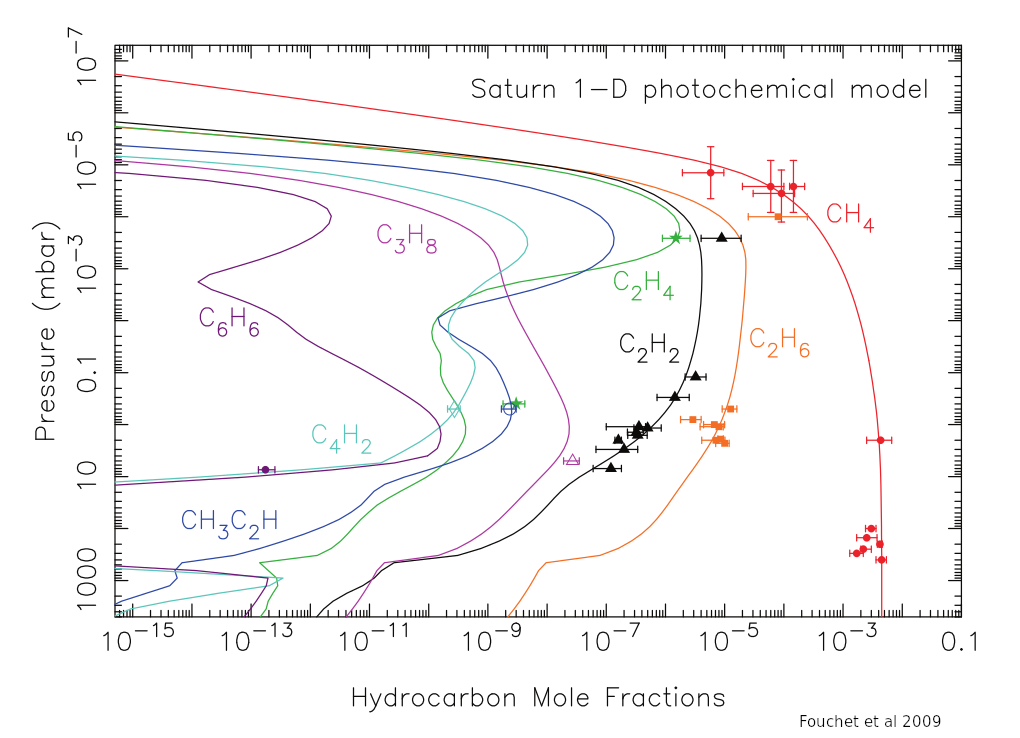
\includegraphics[width=\textwidth]{figs/Fouchet09.png}

\caption{
\footnotesize
Figure taken from \cite{Fouchet2009}. Hydrocarbon mole fractions as a function of
pressure in Saturn's upper atmosphere as derived from the "Model C" 1-D
steady-state photochemical model of \cite{Moses2005}. The solid curves represent
the model profiles for the individual hydrocarbons (as labeled), and the
symbols with associated error bars represent current infrared and ultraviolet
observations. Methane is created in the troposphere and diffuses upwards to the
homopause and the thermosphere where it is photochemically destroyed. Ethane
and acetylene are produced at around \tdex{-4} mbar and diffuse down to the
troposphere where they are converted back to methane. This is the methane cycle
described in \cite{Strobel1969}
}

\label{fig:FouchetPlot}
\end{figure*}

As noted by \cite{Fouchet2009}, important byproducts of these multiple profiles
will be a better determination of the altitude of the CH$_4$ homopause on
Saturn (which is known to be quite variable with latitude from UV occultations
\citealp{Koskinen2018}). This is a function of the rate of
photochemistry, which destroys CH$4$ in the upper atmosphere \citep{Fouchet2009},
and the speed of zonal winds in the stratosphere which distort the shape of the
planet through the centrifugal force \citep{Merritt2019}. 

Photodissociated methane is partially converted into ethane on its way to
becoming aerosols composed of higher order hydrocarbons. Chemical abundances in
the stratosphere impact the thermal profile of the entire atmosphere since
trace gasses are the major absorbers of radiation from the sun and Saturn's
blackbody emissions from lower levels. The proposed analysis will constrain
both the methane and ethane mixing ratios, giving us insight into seasonal
variations in photochemistry and eddy-diffusion rates that we can compare to
models such as those described in \cite{Moses2005}.

Photochemistry also leads to aerosol production. Although not very spectrally
active in our observations, aerosols are thought to be chemically important as
a factor in cloud formation because they sediment downwards to serve as
cloud-condensation nuclei for condensible volatiles in the troposphere
\citep{Fletcher2018}. We will constrain photochemistry and eddy-diffusion rates
through a direct measurement of the relative mixing ratios of methane to
ethane, which will help future investigators understand aerosol production in
the thermosphere and cloud formation processes in the convective regions of the
troposphere. We will measure these abundances with high radial resolution over
the course of nearly half of a Saturnian year at a multitude of latitudes
thanks to \Cas's long-lasting mission in the Saturn system.

Finally, uncertainties in the production and optical properties of
photochemical haze are a major stumbling blocks in current hot-Jupiter
exoplanet atmospheric models and retrievals, as they are thought to be the
cause of the flattening of the transit spectra of gaseous exoplanets
\citep{Fraine2013}.  Through providing a ground-truth
understanding of the atmosphere of one of our local giant planets whose
atmospheric chemistry is also photochemically driven, our analysis will help
future studies constrain the atmospheres of these exciting bodies that we will
soon be able to probe in greater detail with the James Webb Space Telescope,
ELT-class ground-based telescopes, and other future telescopes.


\subsection{The Data: A Part of the Suite of Cassini Stellar Occultation Studies} \label{sec:intro-data}

During the 13-year Cassini mission, the spacecraft observed over 100
occultations of stars by Saturn using the Visual and Infrared Mapping
Spectrometer (VIMS) instrument. These occultations probe Saturn’s atmosphere
between pressures of $\approx$20 $\mu$bar and $\approx$5 mbar. Extinction of light from these stars
is driven primarily by differential refraction and molecular absorption by
hydrocarbons (chiefly CH$_4$ and C$_2$H$_6$). We have proposed to tackle three
scientific projects using these data: (1) to verify the seasonal and
latitudinal temperature maps of Saturn’s stratosphere generated by the Cassini
Composite Infrared Spectrometer (CIRS) by \citealp{Fletcher2007} at higher
radial resolution, (2) to measure the altitude of the methane homopause from
the dropoff of methane abundance with altitude, and (3) to test theoretical
models of Saturn's photochemistry and eddy-diffusion rates \citep{Moses2005}. Our
results for Saturn's atmosphere should complement similar analyses of VIMS
solar occultation data for Titan by Maltagliati et al.  (2015) and Bellucci et
al. (2009).

A handful of these $\approx$100 occultation observations were observed through
a series of small-frame images instead of a single spatial pixel pointed at the
star's initial location on the sky.  These imaging-mode occultations provide a
chance to directly observe the stars' refraction through the outer layers of
Saturn's atmosphere and constrain the relative importance of differential
refraction to other sources of attenuation in the photometry of an occultation.
This is an important calibration for the higher-radial-resolution
occultation-mode data, for which the image of the star much more quickly gets
refracted out of the field of view. This paper focuses on these imaging
occultation experiments and relevant instrumental calibrations.

TODO: Describe each of the six useful imaging-mode occultations. Two are 8x8
low-res. Two are 16x6 hi-res. Two are 16x4 hi-res. Describe geometry, vperp,
and the angle that the star's image gets refracted relative to the X axis.
Put all of this in a table, maybe include a figure.

\section{Data Reduction} \label{sec:data}
The data reduction requires four major steps.

First comes initial background subtractions and 5-$\sigma$ clipping to mask out
erroneous points (one experiment has a cosmic ray strike that messes up
centering and flux calibration).

Second is locating the center of the star in each frame as it is refracted
across the Field of View. This is complicated because the PSF of a star is
smaller than a pixel in the X direction. A two-step centering process described
in two subsections below. The first step is to use PRF scans to map subpixel
sensitivity. The second step is to use the relative brightness of neighboring
pixels to calculate the subpixel stellar center location.

Third is correcting out a limb model of background light from Saturn. Using the
star centers, and knowing that the stellar image tracks the limb of the planet,
we know where the limb of Saturn is. Using rows of pixels far from the star
image, we calculate the variable background associated with Saturn's limb.

Fourth is using the subpixel sensitivity variations and the stellar centers to
calculate the "true" flux of the star, including light that falls in the gaps
between pixels.

\subsection{initial background corrections}
Task 1

\subsection{Center Finding via Subpixel Sensitivity}

\begin{figure*}[ht]
  \centering
  \includegraphics[width=0.95\textwidth]{figs/codeplot.png}
  \caption{Lightcurve and centering results for an occultation of AlpOri
(Betelgeuse) on orbit 271, observed in the 2.7~$\mu$m continuum band. The top
plot displays the flux dropping and twinkling through the atmosphere. The
bottom plot displays the pixel that the majority of starlight in (green),
subpixel centering using the light spilling into a neighboring pixel (red),
and a comparison with a line of slope matching the spacecraft's velocity perpendicular
to the planet's limb (black).  This is one of four types of plots produced by
the code.}
  \label{fig:codeplots}
\end{figure*}

Tracking the center of a star in a VIMS image is a difficult task because the
PSF of the star is less than one pixel. Still, the star is rarely centered in a
pixel, and so centering can be achieved by looking at how much light spills
into the neighbors of the brightest pixel. Fortunately, the Pixel Response
Function (PRF) is well-defined for the single VIMS spatial pixel as a function
of the angle between the center of the pixel and the star. This has been done
by slewing the spacecraft so that the star AlpOri (Betelgeuse) raster-scans
across the pixel. From these, we can calculate the theoretical relative
brightnesses of the pixels on either side of the brightest pixel relative to
the brightest pixel, and compare this to the measured value in the VIMS frame.

First, we must determine which two pixels share the most starlight. To do so,
we:
\begin{enumerate}
  \item integrate over a continuum bandpass to improve signal to noise (e.g. 2.53-2.85 microns)
  \item perform a boxcar smoothing in time (usually 10 frames)
  \item record the brightest pixel for each resulting timestep
  \item locate "transition times" when the brightest pixel changes from one timestep to the next
  \item at each timestep select the brightest pixel and the brightest pixel on the other side of the nearest "trans
ition"
\end{enumerate}

We measure the direction to the star by taking the ratio ($R_{data}$) of the
measured flux in these two selected pixels.  We compare this ratio to the same
ratio calculated from the PRF scans $R_{scans}(t)$ at each time step $t$.  We
calculate the value of $t=t_0$ for which $\chi^2 = (R_{data}-R_{scans}(t_0))^2$
is minimized, and then calculate $\theta(t_0)$ which is the offset of the star
from the center of the pixel at $t_0$.

This metric has many properties which make it useful. Theoretically, it should
be monotonically increasing or decreasing as the star moves steadily in pixel
position.  For PSFs smaller than a pixel, there will be a plateau at zero where
there is no light observed in the neighboring pixel. Away from this plateau
(near the pixel boundaries) we have the best sensitivity to the position of the
star. At metric values $R = 1$ the center of the star's PSF straddles the
boundary with the neighboring pixel and we have the most sensitivity.

{\bf The current version of the code performs fits in each direction independently,
and using manually-selected PRF scan track numbers. A planned improvement is to
fit both simultaneously, which will allow the algorithm to self-select the best
track for each direction.}

After this step, we have occultation profiles in the same form as the
occultation-mode data. This ends the imaging-mode specific portion of the code.
The following two subsections describe code that will be run on all occultation
data.

\subsection{creating and correcting out limb model}
Task 2

\subsection{calculating total observed flux}
Task 3

\section{Results}

Can the flux observed in continuum wavelengths be described by refraction alone, or will there be
haze absorption that we will need to correct out of the occultation-mode data? Can we see a feature
at 2.7 \micron indicating an observation of ring rain? Preliminary Methane-Ethane abundances?
Seasonal and latitudinal variations?

\section{CONCLUSIONS}

In conclusion, we have done some cool science.

\begin{acknowledgments}
Thank you Phil for helping me return to graduate school.
\end{acknowledgments}

\vspace{5mm}
\facilities{Cornell and Cassini}
\software{numpy, scipy, matplotlib, pysis, etc}

\appendix
\section{Gory Details}

Here we present the gory details of how we did science.

\bibliography{imagingoccs.bib}
\bibliographystyle{aasjournal}

\end{document}
